\documentclass[aspectratio=169,11pt,svgnames,handout]{beamer}

\usepackage[english]{babel}
\usepackage{graphicx}
\usepackage{enumitem}
\usepackage{amsmath}
\usepackage{mathtools}
\usepackage{float}
\usepackage{tikz}
\usetikzlibrary{patterns,arrows.meta,calc}
\usepackage{tkz-euclide}
\tikzset{point style/.style = {%
  draw = black,
  inner sep = 0pt,
  shape = circle,
  minimum size = 5pt,
  fill = black
 }
}
\usepackage{enumitem}

\usepackage{caption}
\usepackage{subcaption}

% Flowchart stuff

\usepackage{pgfopts}
\usepackage{xcolor}
\usepackage{tcolorbox}

\usetheme[
 titlestyle=style2,
 titleformat=smallcaps,
 sectionstyle=plain,
 slidestyle=cyber,
 headingcolor=theme,
 block=transparent
]{trigon}

\title{Polygons}
\date{\today}
\author{Adam Klepáč}
\institute[GEVO]{Gymnázium Evolution Jižní Město}
\biglogo[width=.2\textwidth]{logo}
\smalllogo[width=.1\textwidth]{logo}
\titlegraphic{
\includegraphics[height=\paperheight]{title.jpg}}

\def\subsectionname{}

% enumerate global settings
\setlist[enumerate,1]{label=\arabic*.}
\setlist[enumerate,2]{label=\alph*)}

% custom colors %
\definecolor{PolygonYellow}{HTML}{f6e01a}
\definecolor{PolygonCyan}{HTML}{11cdef}
\definecolor{PolygonOrange}{HTML}{b25c10}
\definecolor{PolygonBlue}{HTML}{0a2a66}
\colorlet{tPrim}{PolygonBlue}
\colorlet{tTheme}{PolygonYellow}
\colorlet{tSec}{PolygonCyan}
\colorlet{tAccent}{PolygonCyan}

\newcommand{\clc}{\textcolor{PolygonCyan}}
\newcommand{\clb}{\textcolor{PolygonBlue}}
\newcommand{\clo}{\textcolor{PolygonOrange}}

\tcbset{
 boxsep=7pt,
 fonttitle=\sc,
 colframe=tGreyBg,
 colframe=tPrim,
 boxrule=1pt
}

\begin{document}
\titleframe

\begin{frame}
 \frametitle{Contents}
 \tableofcontents
\end{frame}

\section{General Polygons}
\label{sec:general-polygons}

\begin{frame}
 \frametitle{General Polygons -- Def~\hspace{-.4ex}inition}
 \begin{tcolorbox}[title=Polygon]
  A \alert{polygon} is a closed 2D shape made of only segments.
 \end{tcolorbox}
 \begin{itemize}
  \item<2-> The endpoints of those segments are called \alert{vertices}.
  \item<3-> The segments themselves are called \alert{edges}.
 \end{itemize}
\end{frame}

\begin{frame}
 \frametitle{General Polygons -- Examples}
 \begin{figure}[H]
  \centering
  \begin{subfigure}[b]{.23\textwidth}
   \centering
   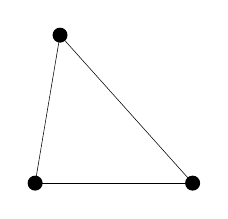
\begin{tikzpicture}
    \tkzDefPoint(0:1){A}
    \tkzDefPoint(110:2){B}
    \tkzDefPoint(180:1){C}

    \tkzDrawPoints(A,B,C);
    \tkzDrawSegments(A,B B,C C,A);
   \end{tikzpicture}
   \caption*{Triangle}
  \end{subfigure}
  \begin{subfigure}[b]{.23\textwidth}
   \centering
   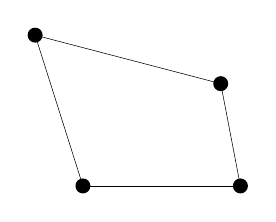
\begin{tikzpicture}
    \tkzDefPoint(0:1){A}
    \tkzDefPoint(60:1.5){B}
    \tkzDefPoint(130:2.5){C}
    \tkzDefPoint(180:1){D}

    \tkzDrawPoints(A,B,C,D);
    \tkzDrawSegments(A,B B,C C,D D,A);
   \end{tikzpicture}
   \caption*{Quadrilateral}
  \end{subfigure}
  \begin{subfigure}[b]{.23\textwidth}
   \centering
   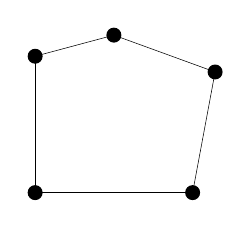
\begin{tikzpicture}
    \tkzDefPoint(0:1){A}
    \tkzDefPoint(50:2){B}
    \tkzDefPoint(90:2){C}
    \tkzDefPoint(120:2){D}
    \tkzDefPoint(180:1){E}

    \tkzDrawPoints(A,B,C,D,E);
    \tkzDrawSegments(A,B B,C C,D D,E E,A);
   \end{tikzpicture}
   \caption*{Pentagon}
  \end{subfigure}
  \begin{subfigure}[b]{.27\textwidth}
   \centering
   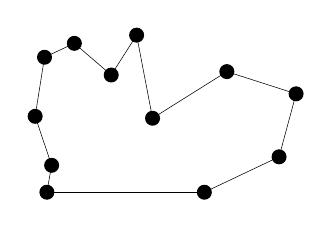
\begin{tikzpicture}
    \tkzDefPoint(0:1){A}
    \tkzDefPoint(13:2){B}
    \tkzDefPoint(30:2.5){C}
    \tkzDefPoint(50:2){D}
    \tkzDefPoint(70:1){E}
    \tkzDefPoint(86:2){F}
    \tkzDefPoint(97:1.5){G}
    \tkzDefPoint(109:2){H}
    \tkzDefPoint(121:2){I}
    \tkzDefPoint(140:1.5){J}
    \tkzDefPoint(160:1){K}
    \tkzDefPoint(180:1){L}

    \tkzDrawPoints(A,B,C,D,E,F,G,H,I,J,K,L);
    \tkzDrawSegments(A,B B,C C,D D,E E,F F,G G,H H,I I,J J,K K,L L,A);
   \end{tikzpicture}
   \caption*{Dodecagon}
  \end{subfigure}
 \end{figure}
 \begin{itemize}
  \item <2-> A polygon with $n \in \mathbb{N}$ sides is called an $n$-gon.
  \item <3-> For example a polygon with 123456 sides is called a $123456$-gon or
   decadismyriatrischilliatetrahectapentacontakaihexagon.
 \end{itemize} 
\end{frame}

\begin{frame}
 \frametitle{General Polygons -- Counterexamples}
 \begin{figure}[H]
  \centering
  \begin{subfigure}[b]{.33\textwidth}
   \centering
   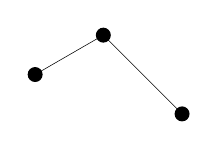
\begin{tikzpicture}
    \tkzDefPoint(0:1){A}
    \tkzDefPoint(90:1){B}
    \tkzDefPoint(150:1){C}

    \tkzDrawPoints(A,B,C);
    \tkzDrawSegments(A,B B,C);
   \end{tikzpicture}
   \caption*{Not closed}
  \end{subfigure}
  \begin{subfigure}[b]{.33\textwidth}
   \centering
   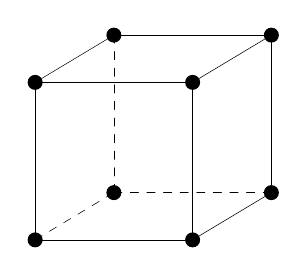
\begin{tikzpicture}[scale=2]
    \tkzDefPoint(0,0){A1}
    \tkzDefPoint(0,1){B1}
    \tkzDefPoint(1,1){C1}
    \tkzDefPoint(1,0){D1}

    \tkzDefPoint(0.5,0.3){A2}
    \tkzDefPoint(0.5,1.3){B2}
    \tkzDefPoint(1.5,1.3){C2}
    \tkzDefPoint(1.5,0.3){D2}
    \tkzDrawPoints(A1,B1,C1,D1,A2,B2,C2,D2)

    \tkzDrawSegments(A1,B1 B1,C1 C1,D1 D1,A1 B2,C2 C2,D2 B1,B2 C1,C2 D1,D2)
    \tkzDrawSegments[dashed](A2,B2 D2,A2 A1,A2)
   \end{tikzpicture}
   \caption*{3D}
  \end{subfigure}
  \begin{subfigure}[b]{.33\textwidth}
   \centering
   \begin{tikzpicture}
    \tkzDefPoint(0:1){A}
    \tkzDefPoint(180:1){B}
    \tkzDefPoint(90:1){P}

    \tkzDrawPoints(A,B)
    \tkzDrawArc(P,A)(B)
    \tkzDrawSegment(A,B)
   \end{tikzpicture}
   \caption*{Not straight}
  \end{subfigure}
 \end{figure}
\end{frame}

\begin{frame}
 \frametitle{General Polygons -- Convexity}
 \begin{tcolorbox}[title=Convex Polygon]
  A polygon is called \alert{convex} if it has no internal angle greater than
  180$^{\circ}$.
 \end{tcolorbox}
 \pause
 \begin{figure}[H]
  \centering
  \begin{subfigure}[b]{.45\textwidth}
   \centering
   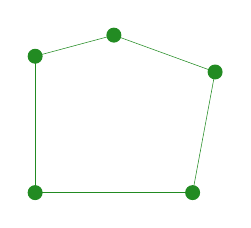
\begin{tikzpicture}
    \tkzDefPoint(0:1){A}
    \tkzDefPoint(50:2){B}
    \tkzDefPoint(90:2){C}
    \tkzDefPoint(120:2){D}
    \tkzDefPoint(180:1){E}

    \tkzDrawPoints[color=ForestGreen](A,B,C,D,E);
    \tkzDrawSegments[color=ForestGreen](A,B B,C C,D D,E E,A);
   \end{tikzpicture}
   \caption*{\textcolor{ForestGreen}{Convex}}
  \end{subfigure}
  \begin{subfigure}[b]{.45\textwidth}
   \centering
   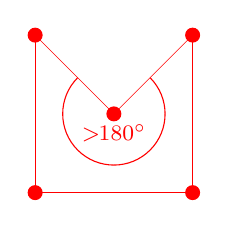
\begin{tikzpicture}
    \tkzDefPoint(0,0){A}
    \tkzDefPoint(2,0){B}
    \tkzDefPoint(2,2){C}
    \tkzDefPoint(1,1){D}
    \tkzDefPoint(0,2){E}

    \tkzDrawPoints[color=Red](A,B,C,D,E)
    \tkzDrawSegments[color=Red](A,B B,C C,D D,E E,A)

    \tkzMarkAngle[color=Red,size=0.65](E,D,C)
    \tkzLabelAngle[color=Red,pos=0.25](E,D,C){\footnotesize $>\!\!180^{ \circ}$}
   \end{tikzpicture}
   \caption*{\textcolor{Red}{NOT convex}}
  \end{subfigure}
 \end{figure}
\end{frame}

\section{Convex Polygons}
\label{sec:convex-polygons}

\begin{frame}
 \frametitle{Convex Polygons -- Special Types}
 \begin{figure}[H]
  \centering
  \begin{subfigure}[b]{.33\textwidth}
   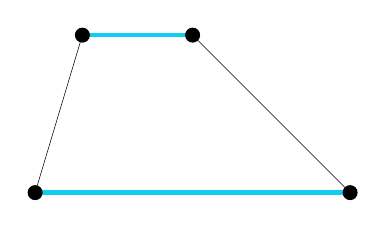
\begin{tikzpicture}[scale=2]
    \tkzDefPoint(0,0){A}
    \tkzDefPoint(0.3,1){B}
    \tkzDefPoint(1,1){C}
    \tkzDefPoint(2,0){D}

    \tkzDrawPolygon(A,B,C,D)
    \tkzDrawSegments[ultra thick,PolygonCyan](B,C A,D)
    \tkzDrawPoints(A,B,C,D)
   \end{tikzpicture}
   \caption*{\alert{Trapezoid/Trapezium}\\
    A convex quadrilateral with at least two
   parallel sides.}
  \end{subfigure}
  \pause
  \begin{subfigure}[b]{.33\textwidth}
   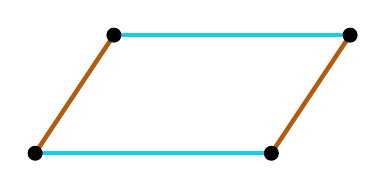
\begin{tikzpicture}[scale=2]
    \tkzDefPoint(0,0){A}
    \tkzDefPoint(0.5,0.75){B}
    \tkzDefPoint(2,0.75){C}
    \tkzDefPoint(1.5,0){D}

    \tkzDrawSegments[ultra thick,PolygonCyan](B,C A,D)
    \tkzDrawSegments[ultra thick,PolygonOrange](A,B C,D)
    \tkzDrawPoints(A,B,C,D)
   \end{tikzpicture}
   \caption*{\alert{Parallelogram}\\
    A convex quadrilateral with two pairs of
   parallel sides.}
  \end{subfigure}
  \pause
  \begin{subfigure}[b]{.33\textwidth}
   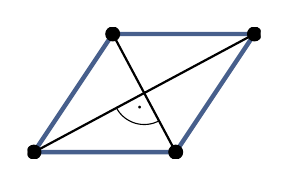
\begin{tikzpicture}[scale=2]
    \clip (-0.04,-0.04) rectangle (1.44,0.79);
    \tkzDefPoint(0,0){A}
    \tkzDefPoint(0.5,0.75){B}
    \tkzDefPoint(1.4,0.75){C}
    \tkzDefPoint(0.9,0){D}

    \tkzDrawPolygon[ultra thick,PolygonBlue!75](A,B,C,D)
    \tkzDrawPoints(A,B,C,D)
    \tkzDrawSegments[thick](A,C B,D)
    \tkzInterLL(A,C)(B,D) \tkzGetPoint{O}
    \tkzMarkAngle[size=0.2](A,O,D)
    \tkzLabelAngle[pos=0.1](A,O,D){$ \cdot $}
   \end{tikzpicture}
   \caption*{\alert{Rhombus}\\
   An \textbf{equilateral} (all sides of the same length) parallelogram.}
  \end{subfigure}
 \end{figure}
\end{frame}

\begin{frame}
 \frametitle{Convex Polygons -- Diagonals}
 \begin{tcolorbox}[title=Diagonal in A Convex Polygon]
  A \alert{diagonal} of a \textbf{convex} polygon is a segment connecting two of
  its non-adjacent vertices.
 \end{tcolorbox}
 \begin{minipage}[c][4cm][c]{0.48\textwidth}
  \begin{figure}[H]
   \centering
   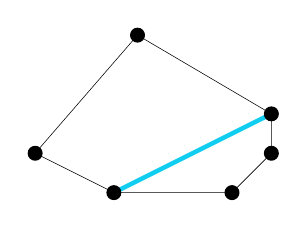
\begin{tikzpicture}
    \tkzDefPoint(0,0){A}
    \tkzDefPoint(-1,0.5){B}
    \tkzDefPoint(0.3,2){C}
    \tkzDefPoint(2,1){D}
    \tkzDefPoint(2,0.5){E}
    \tkzDefPoint(1.5,0){F}
    \tkzDrawPolygon(A,B,C,D,E,F)
    \tkzDrawSegment[color=PolygonCyan,ultra thick](A,D)
    \tkzDrawPoints(A,B,C,D,E,F)
   \end{tikzpicture}
   \caption*{\textcolor{PolygonCyan}{Diagonal} in a convex hexagon.}
  \end{figure}
 \end{minipage}
 \pause
 \begin{minipage}[c][4cm][c]{.48\textwidth}
  \vspace*{\fill}
  \textcolor{PolygonOrange}{\textbf{Voluntary HW}}: How many different diagonals
  does a convex $n$-gon have?
  \vspace*{\fill}
 \end{minipage}
\end{frame}

\begin{frame}
 \frametitle{Convex Polygons -- Triangulations}
 \begin{tcolorbox}[title=Triangulation of A Convex Polygon]
  A \alert{triangulation} of a \textbf{convex} polygon is its division into
  triangles by non-intersecting diagonals.
 \end{tcolorbox}
 \pause
 \begin{figure}[H]
  \centering
  \begin{subfigure}[b]{.2\textwidth}
   \centering
   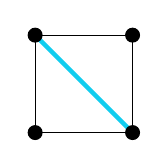
\begin{tikzpicture}[scale=0.875]
    \tkzDefPoint(-45:1){A}
    \tkzDefPoint(-135:1){B}
    \tkzDefPoint(135:1){C}
    \tkzDefPoint(45:1){D}

    \tkzDrawPolygon(A,B,C,D)
    \tkzDrawSegment[ultra thick,PolygonCyan](A,C)
    \tkzDrawPoints(A,B,C,D)
   \end{tikzpicture}
  \end{subfigure}
  \begin{subfigure}[b]{.2\textwidth}
   \centering
   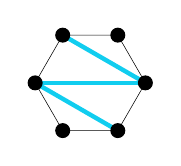
\begin{tikzpicture}[scale=0.7]
    \tkzDefPoint(0:1){A}
    \tkzDefPoint(60:1){B}
    \tkzDefPoint(120:1){C}
    \tkzDefPoint(180:1){D}
    \tkzDefPoint(240:1){E}
    \tkzDefPoint(300:1){F}

    \tkzDrawPolygon(A,B,C,D,E,F)
    \tkzDrawSegments[ultra thick,color=PolygonCyan](A,C D,F A,D)
    \tkzDrawPoints(A,B,C,D,E,F)
   \end{tikzpicture}
  \end{subfigure}
  \begin{subfigure}[b]{.2\textwidth}
   \centering
   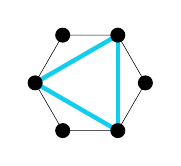
\begin{tikzpicture}[scale=0.7]
    \tkzDefPoint(0:1){A}
    \tkzDefPoint(60:1){B}
    \tkzDefPoint(120:1){C}
    \tkzDefPoint(180:1){D}
    \tkzDefPoint(240:1){E}
    \tkzDefPoint(300:1){F}

    \tkzDrawPolygon(A,B,C,D,E,F)
    \tkzDrawSegments[ultra thick,color=PolygonCyan](B,D D,F B,F)
    \tkzDrawPoints(A,B,C,D,E,F)
   \end{tikzpicture}
  \end{subfigure}
  \caption*{Examples of \textcolor{PolygonCyan}{triangulations}.}
 \end{figure}
 \vspace*{-1em}
 \pause
 \textcolor{PolygonOrange}{\textbf{Voluntary HW}}: How many different
 triangulations of an $n$-gon are there?
\end{frame}

\begin{frame}
 \frametitle{Convex Polygons -- Triangulations}
 \begin{tcolorbox}[title=Triangulation of A Convex Polygon]
  A \alert{triangulation} of a \textbf{convex} polygon is its division into
  triangles by non-intersecting diagonals.
 \end{tcolorbox}
 \begin{figure}[H]
  \centering
  \begin{subfigure}[b]{.2\textwidth}
   \centering
   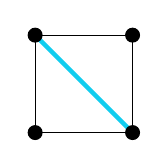
\begin{tikzpicture}[scale=0.875]
    \tkzDefPoint(-45:1){A}
    \tkzDefPoint(-135:1){B}
    \tkzDefPoint(135:1){C}
    \tkzDefPoint(45:1){D}

    \tkzDrawPolygon(A,B,C,D)
    \tkzDrawSegment[ultra thick,PolygonCyan](A,C)
    \tkzDrawPoints(A,B,C,D)
   \end{tikzpicture}
  \end{subfigure}
  \begin{subfigure}[b]{.2\textwidth}
   \centering
   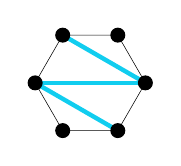
\begin{tikzpicture}[scale=0.7]
    \tkzDefPoint(0:1){A}
    \tkzDefPoint(60:1){B}
    \tkzDefPoint(120:1){C}
    \tkzDefPoint(180:1){D}
    \tkzDefPoint(240:1){E}
    \tkzDefPoint(300:1){F}

    \tkzDrawPolygon(A,B,C,D,E,F)
    \tkzDrawSegments[ultra thick,color=PolygonCyan](A,C D,F A,D)
    \tkzDrawPoints(A,B,C,D,E,F)
   \end{tikzpicture}
  \end{subfigure}
  \begin{subfigure}[b]{.2\textwidth}
   \centering
   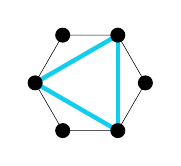
\begin{tikzpicture}[scale=0.7]
    \tkzDefPoint(0:1){A}
    \tkzDefPoint(60:1){B}
    \tkzDefPoint(120:1){C}
    \tkzDefPoint(180:1){D}
    \tkzDefPoint(240:1){E}
    \tkzDefPoint(300:1){F}

    \tkzDrawPolygon(A,B,C,D,E,F)
    \tkzDrawSegments[ultra thick,color=PolygonCyan](B,D D,F B,F)
    \tkzDrawPoints(A,B,C,D,E,F)
   \end{tikzpicture}
  \end{subfigure}
  \caption*{Examples of \textcolor{PolygonCyan}{triangulations}.}
 \end{figure}
 \vspace*{-1em}
 \textcolor{PolygonOrange}{\textbf{Voluntary HW}}: Find a \textbf{non-convex}
 polygon which \textbf{cannot} be triangulated.
\end{frame}

\begin{frame}
 \frametitle{Convex Polygons -- Internal Angles}
 \begin{figure}[H]
  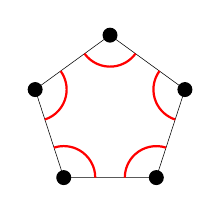
\begin{tikzpicture}
   \tkzDefPoint(-54:1){A};
   \tkzDefPoint(18:1){B};
   \tkzDefPoint(90:1){C};
   \tkzDefPoint(162:1){D};
   \tkzDefPoint(234:1){E};

   \tkzDrawPolygon(A,B,C,D,E);
   \tkzDrawPoints(A,B,C,D,E);
   \tkzMarkAngle[size=0.4,Red,thick](B,A,E)
   \tkzMarkAngle[size=0.4,Red,thick](A,E,D)
   \tkzMarkAngle[size=0.4,Red,thick](E,D,C)
   \tkzMarkAngle[size=0.4,Red,thick](D,C,B)
   \tkzMarkAngle[size=0.4,Red,thick](C,B,A)
  \end{tikzpicture}
  \caption*{\textcolor{Red}{\textbf{Internal angles}} of a pentagon.}
 \end{figure}
 \textbf{Question:} What is the sum of internal angles of a convex $n$-gon?
 \begin{itemize}[label=\textbullet]
  \item<2-> For a triangle, it's 180$^{ \circ }$.
  \item<3-> For a square, it's 360$^{\circ}$.
  \item<4-> For a pentagon, it's 540$^{ \circ }$.
 \end{itemize}
\end{frame}

\begin{frame}
 \frametitle{Convex Polygons -- Internal Angles}
 \begin{itemize}
  \item We can count internal angles using triangulations.
  \pause
  \item Into how many triangles is a convex $n$-gon divided?
  \pause
  \item Each triangle shares two vertices with an adjacent one.
  \pause
  \item We choose the first triangle -- it covers 3 vertices.
  \pause
  \item After that, each triangle covers only one more vertex.
  \pause
  \item This means, that an $n$-gon is divided into $n-2$ triangles.
 \end{itemize}
 \begin{figure}[H]
  \pause
  \begin{subfigure}[b]{.24\textwidth}
   \centering
   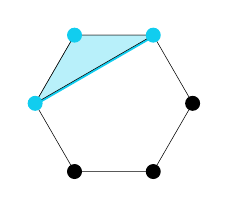
\begin{tikzpicture}
    \tkzDefPoint(0:1){A}
    \tkzDefPoint(60:1){B}
    \tkzDefPoint(120:1){C}
    \tkzDefPoint(180:1){D}
    \tkzDefPoint(240:1){E}
    \tkzDefPoint(300:1){F}

    \tkzDrawPolygon(A,B,C,D,E,F)
    \tkzDrawSegment[ultra thick,color=PolygonCyan](B,D)
    \tkzDrawPolygon[fill=PolygonCyan!30](B,C,D)
    \tkzDrawPoints(A,E,F)
    \tkzDrawPoints[color=PolygonCyan](B,C,D)
   \end{tikzpicture}
  \end{subfigure}
  \begin{subfigure}[b]{.24\textwidth}
   \centering
   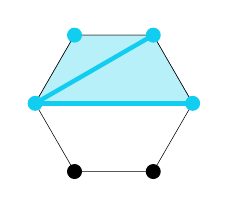
\begin{tikzpicture}
    \tkzDefPoint(0:1){A}
    \tkzDefPoint(60:1){B}
    \tkzDefPoint(120:1){C}
    \tkzDefPoint(180:1){D}
    \tkzDefPoint(240:1){E}
    \tkzDefPoint(300:1){F}

    \tkzDrawPolygon(A,B,C,D,E,F)
    \tkzDrawPolygon[fill=PolygonCyan!30](B,C,D)
    \tkzDrawPolygon[fill=PolygonCyan!30](A,B,D)
    \tkzDrawSegment[ultra thick,color=PolygonCyan](B,D)
    \tkzDrawSegment[ultra thick,color=PolygonCyan](A,D)
    \tkzDrawPoints(E,F)
    \tkzDrawPoints[color=PolygonCyan](A,B,C,D)
   \end{tikzpicture}
  \end{subfigure}
  \begin{subfigure}[b]{.24\textwidth}
   \centering
   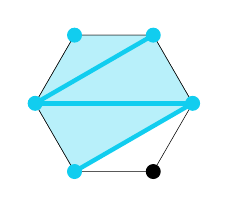
\begin{tikzpicture}
    \tkzDefPoint(0:1){A}
    \tkzDefPoint(60:1){B}
    \tkzDefPoint(120:1){C}
    \tkzDefPoint(180:1){D}
    \tkzDefPoint(240:1){E}
    \tkzDefPoint(300:1){F}

    \tkzDrawPolygon(A,B,C,D,E,F)
    \tkzDrawPolygon[fill=PolygonCyan!30](B,C,D)
    \tkzDrawPolygon[fill=PolygonCyan!30](A,B,D)
    \tkzDrawPolygon[fill=PolygonCyan!30](A,D,E)
    \tkzDrawSegment[ultra thick,color=PolygonCyan](B,D)
    \tkzDrawSegment[ultra thick,color=PolygonCyan](A,D)
    \tkzDrawSegment[ultra thick,color=PolygonCyan](A,E)
    \tkzDrawPoints(F)
    \tkzDrawPoints[color=PolygonCyan](A,B,C,D,E)
   \end{tikzpicture}
  \end{subfigure}
  \begin{subfigure}[b]{.24\textwidth}
   \centering
   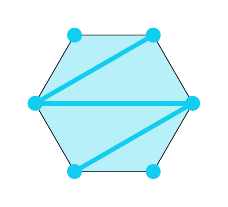
\begin{tikzpicture}
    \tkzDefPoint(0:1){A}
    \tkzDefPoint(60:1){B}
    \tkzDefPoint(120:1){C}
    \tkzDefPoint(180:1){D}
    \tkzDefPoint(240:1){E}
    \tkzDefPoint(300:1){F}

    \tkzDrawPolygon(A,B,C,D,E,F)
    \tkzDrawPolygon[fill=PolygonCyan!30](B,C,D)
    \tkzDrawPolygon[fill=PolygonCyan!30](A,B,D)
    \tkzDrawPolygon[fill=PolygonCyan!30](A,D,E)
    \tkzDrawPolygon[fill=PolygonCyan!30](A,E,F)
    \tkzDrawSegment[ultra thick,color=PolygonCyan](B,D)
    \tkzDrawSegment[ultra thick,color=PolygonCyan](A,D)
    \tkzDrawSegment[ultra thick,color=PolygonCyan](A,E)
    \tkzDrawPoints[color=PolygonCyan](A,B,C,D,E,F)
   \end{tikzpicture}
  \end{subfigure}
  \caption*{Construction of a \textcolor{PolygonCyan}{triangulation} of a
  hexagon.}
 \end{figure}
\end{frame}

\begin{frame}
 \frametitle{Convex Polygons -- Internal Angles}
 \begin{itemize}
  \item A convex $n$-gon is divided into $n-2$ triangles.
  \pause
  \item The sum of all internal angles in a triangle is 180$^{ \circ }$.
 \end{itemize}
 \pause
 \begin{tcolorbox}[title=Sum of Internal Angles in a Convex Polygon]
  The sum of all internal angles of a convex $n$-gon is $(n-2) \cdot 180^{ \circ
  }$.
 \end{tcolorbox}
\end{frame}

\section{Regular Polygons}

\begin{frame}
 \frametitle{Def~\hspace*{-.4ex}inition}
 \begin{tcolorbox}[title=Regular Polygon]
  A \alert{regular polygon} is a convex polygon whose sides all have the same
  length and whose internal angles all have the same size.
 \end{tcolorbox}
 \pause
 \begin{figure}[H]
  \captionsetup{justification=centering}
  \centering
  \begin{subfigure}[t]{.24\textwidth}
   \centering
   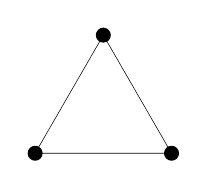
\begin{tikzpicture}
    \tkzDefPoint(-30:1){A}
    \tkzDefPoint(90:1){B}
    \tkzDefPoint(210:1){C}
     
    \tkzDrawPolygon(A,B,C)
    \tkzDrawPoints(A,B,C)
   \end{tikzpicture}
   \caption*{Equilateral triangle (regular trigon)}
  \end{subfigure}
  \begin{subfigure}[t]{.24\textwidth}
   \centering
   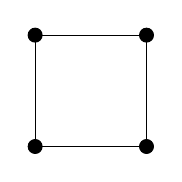
\begin{tikzpicture}
    \tkzDefPoint(-45:1){A}
    \tkzDefPoint(-135:1){B}
    \tkzDefPoint(135:1){C}
    \tkzDefPoint(45:1){D}
     
    \tkzDrawPolygon(A,B,C,D)
    \tkzDrawPoints(A,B,C,D)
   \end{tikzpicture}
   \caption*{Square (regular tetragon)}
  \end{subfigure}
  \begin{subfigure}[t]{.24\textwidth}
   \centering
   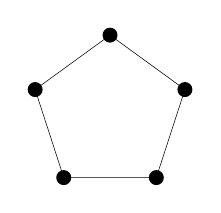
\begin{tikzpicture}
    \tkzDefPoint(-54:1){A}
    \tkzDefPoint(18:1){B}
    \tkzDefPoint(90:1){C}
    \tkzDefPoint(162:1){D}
    \tkzDefPoint(234:1){E}
     
    \tkzDrawPolygon(A,B,C,D,E)
    \tkzDrawPoints(A,B,C,D,E)
   \end{tikzpicture}
   \caption*{Regular pentagon}
  \end{subfigure}
  \begin{subfigure}[t]{.24\textwidth}
   \centering
   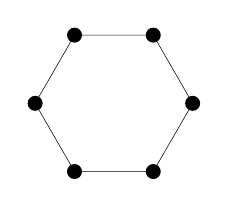
\begin{tikzpicture}
    \tkzDefPoint(0:1){A}
    \tkzDefPoint(60:1){B}
    \tkzDefPoint(120:1){C}
    \tkzDefPoint(180:1){D}
    \tkzDefPoint(240:1){E}
    \tkzDefPoint(300:1){F}
     
    \tkzDrawPolygon(A,B,C,D,E,F)
    \tkzDrawPoints(A,B,C,D,E,F)
   \end{tikzpicture}
   \caption*{Regular hexagon}
  \end{subfigure}
 \end{figure}
\end{frame}

\begin{frame}
 \frametitle{Review -- Plane Transformations}
 \begin{tcolorbox}[title=Rotation]
  \alert{Rotation} of a polygon consists of well ... rotating each of
  its points by a fixed angle around a fixed point (called \emph{anchor}).
 \end{tcolorbox}
 \pause
 \begin{figure}[H]
  \centering
  \begin{subfigure}[t]{.3\textwidth}
   \centering
   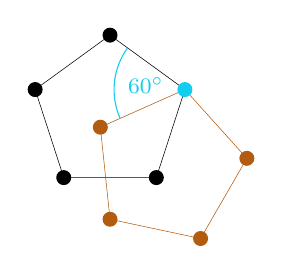
\begin{tikzpicture}
    \foreach \angle/\name in {-54/A,18/B,90/C,162/D,234/E} {
     \tkzDefPoint(\angle:1){\name}
    }
    \tkzDrawPolygon(A,B,C,D,E)
    \tkzDrawPoints(A,D,C,E)
    \tkzDefPointsBy[rotation=center B angle 60](A,B,C,D,E){A',B',C',D',E'}
    \tkzDrawPolygon[color=PolygonOrange](A',B',C',D',E')
    \tkzDrawPoints[color=PolygonOrange](A',C',D',E')
    \tkzDrawPoint[color=PolygonCyan](B)
    \tkzMarkAngle[color=PolygonCyan,size=0.9](C,B,C')
   \tkzLabelAngle[pos=0.5,color=PolygonCyan](C,B,C'){\footnotesize $60^{\circ}$}
   \end{tikzpicture}
  \end{subfigure}
  \begin{subfigure}[t]{.3\textwidth}
   \centering
   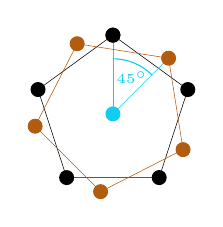
\begin{tikzpicture}
    \foreach \angle/\name in {-54/A,18/B,90/C,162/D,234/E} {
     \tkzDefPoint(\angle:1){\name}
    }
    \tkzDefPoint(0,0){O}
    \tkzDrawPolygon(A,B,C,D,E)
    \tkzDrawPoints(A,B,D,C,E)
    \tkzDrawPoint[color=PolygonCyan](O)
    \tkzDefPointsBy[rotation=center O angle -45](A,B,C,D,E){A',B',C',D',E'}
    \tkzDrawSegments[color=PolygonCyan](O,C O,C')
    \tkzDrawPoint(C)
    \tkzDrawPolygon[color=PolygonOrange](A',B',C',D',E')
    \tkzDrawPoints[color=PolygonOrange](A',B',C',D',E')
    \tkzMarkAngle[color=PolygonCyan,size=0.7](C',O,C)
    \tkzLabelAngle[color=PolygonCyan,pos=0.5,xshift=0.5mm](C',O,C){\tiny $45^{ \circ
    }$}
   \end{tikzpicture}
  \end{subfigure}
  \caption*{Examples of rotations.}
 \end{figure}
\end{frame}

\begin{frame}
 \frametitle{Review -- Plane Transformations}
 \begin{tcolorbox}[title=Ref~\hspace*{-.4ex}lection]
  \alert{Reflection} of a polygon consists of `mirroring' each of its points
  through a given line (called \emph{axis of reflection}).
 \end{tcolorbox}
 \pause
 \begin{figure}[H]
  \centering
  \begin{subfigure}[t]{.3\textwidth}
   \centering
   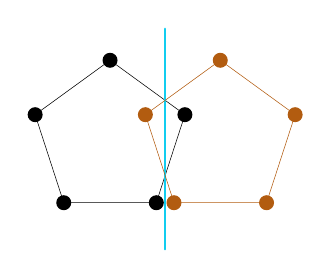
\begin{tikzpicture}
    \foreach \angle/\name in {-54/A,18/B,90/C,162/D,234/E} {
     \tkzDefPoint(\angle:1){\name}
    }
    \tkzDrawPolygon(A,B,C,D,E)
    \tkzDrawPoints(A,B,C,D,E)
    \tkzDefPoints{0.7/1/O,0.7/-1/P}
    \tkzDrawLine[thick,color=PolygonCyan](O,P)
    \tkzDefPointsBy[reflection=over O--P](A,B,C,D,E){A',B',C',D',E'}
    \tkzDrawPolygon[color=PolygonOrange](A',B',C',D',E')
    \tkzDrawPoints[color=PolygonOrange](A',B',C',D',E')
   \end{tikzpicture}
  \end{subfigure}
  \begin{subfigure}[t]{.3\textwidth}
   \centering
   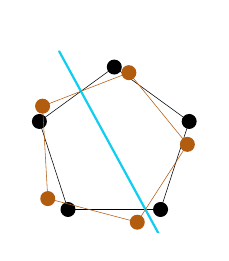
\begin{tikzpicture}
    \clip (-1.1,-1.1) rectangle (1.1,1.5);
    \foreach \angle/\name in {-54/A,18/B,90/C,162/D,234/E} {
     \tkzDefPoint(\angle:1){\name}
    }
    \tkzDrawPolygon(A,B,C,D,E)
    \tkzDrawPoints(A,B,C,D,E)
    \tkzDefPoints{-1/1.75/O,0.5/-1/P}
    \tkzDrawLine[thick,color=PolygonCyan,add=-0.2 and 0.2](O,P)
    \tkzDefPointsBy[reflection=over O--P](A,B,C,D,E){A',B',C',D',E'}
    \tkzDrawPolygon[color=PolygonOrange](A',B',C',D',E')
    \tkzDrawPoints[color=PolygonOrange](A',B',C',D',E')
   \end{tikzpicture}
  \end{subfigure}
  \caption*{Examples of reflections.}
 \end{figure}
\end{frame}

\begin{frame}
 \frametitle{Review -- Plane Transformations}
 \begin{tcolorbox}[title=Point Symmetry]
  \alert{Point symmetry} of a polygon consists of `mirroring' each of its points
  through a given point (called \emph{center of symmetry}).
 \end{tcolorbox}
 \pause
 \begin{figure}[H]
 \centering
 \begin{subfigure}[t]{.3\textwidth}
  \centering
  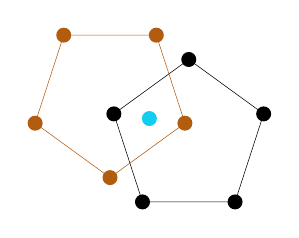
\begin{tikzpicture}
   \foreach \angle/\name in {-54/A,18/B,90/C,162/D,234/E} {
    \tkzDefPoint(\angle:1){\name}
   }
   \tkzDrawPolygon(A,B,C,D,E)
   \tkzDrawPoints(A,B,C,D,E)
   \tkzDefPoint(-0.5,0.25){O}
   \tkzDrawPoint[color=PolygonCyan](O)

   \tkzDefPointsBy[symmetry=center O](A,B,C,D,E){A',B',C',D',E'}
   \tkzDrawPolygon[color=PolygonOrange](A',B',C',D',E')
   \tkzDrawPoints[color=PolygonOrange](A',B',C',D',E')
  \end{tikzpicture}
 \end{subfigure}
 \begin{subfigure}[t]{.3\textwidth}
  \centering
  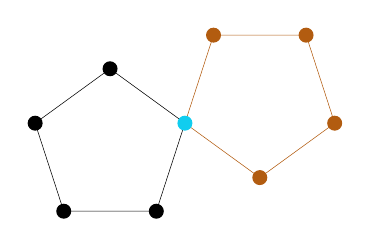
\begin{tikzpicture}
   \foreach \angle/\name in {-54/A,18/B,90/C,162/D,234/E} {
    \tkzDefPoint(\angle:1){\name}
   }
   \tkzDrawPolygon(A,B,C,D,E)
   \tkzDrawPoints(A,C,D,E)

   \tkzDefPointsBy[symmetry=center B](A,B,C,D,E){A',B',C',D',E'}
   \tkzDrawPolygon[color=PolygonOrange](A',B',C',D',E')
   \tkzDrawPoints[color=PolygonOrange](A',C',D',E')
   \tkzDrawPoint[color=PolygonCyan](B)
  \end{tikzpicture}
 \end{subfigure}
 \caption*{Examples of point symmetries.}
\end{figure}
\end{frame}

\begin{frame}
 \frametitle{Symmetries of Regular Polygons}
 \textbf{Question:} What are the transformations that don't change regular
 polygons in any way?
 \pause
 \begin{itemize}[label=\textbullet]
  \item<1-> rotational symmetries
  \begin{itemize}[label=$\circ$]
   \item<2-> rotation by $\frac{k \cdot 360^{ \circ }}{n}$ where $k$ is any
    number between $1$ and $n$
  \end{itemize}
 \item<3-> reflectional (line) symmetries
  \begin{itemize}[label=$\circ$]
   \item<4-> for $n$ even reflections over lines passing through centres of opposite
    sides
   \item<4-> for $n$ even over lines passing through opposite vertices
   \item<4-> for $n$ odd over lines passing through a centre of a side and the
    opposite vertex
  \end{itemize}
 \item<5-> point symmetries
 \begin{itemize}[label=$\circ$]
  \item<6-> only through the `centre' -- the point where its axes of symmetry
   intersect -- in case $n$ is even
 \end{itemize}
 \end{itemize}
\end{frame}

\begin{frame}
 \frametitle{Symmetries of Regular Polygons}
 \begin{figure}[H]
  \centering
  \begin{subfigure}[b]{\textwidth}
   \centering
   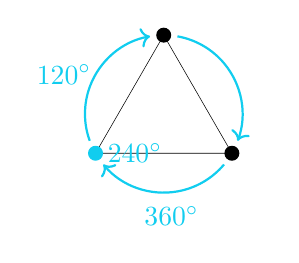
\begin{tikzpicture}
    \foreach \angle/\name in {-30/A,90/B,210/C} {
     \tkzDefPoint(\angle:1){\name}
    }
    \tkzDefPoint(0,0){O}
    \tkzDrawPolygon(A,B,C)
    \tkzDrawPoints(A,B)
    \tkzDrawPoint[color=PolygonCyan](C)
    \tkzDrawArc[color=PolygonCyan,thick,<-,delta=-10](O,B)(C)
    \tkzLabelArc[PolygonCyan,xshift=-4mm](O,B,C){$120^{ \circ }$}
    \tkzDrawArc[color=PolygonCyan,thick,<-,delta=-10](O,A)(B)
    \tkzLabelArc[PolygonCyan,xshift=5mm](O,A,B){$240^{ \circ }$}
    \tkzDrawArc[color=PolygonCyan,thick,<-,delta=-10](O,C)(A)
    \tkzLabelArc[PolygonCyan,yshift=-3mm,xshift=1mm](O,C,A){$360^{ \circ }$}
   \end{tikzpicture}
  \end{subfigure}
  \pause
  \begin{subfigure}[b]{.45\textwidth}
   \centering
   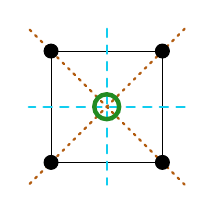
\begin{tikzpicture}
    \foreach \angle/\name in {-45/A,45/B,135/C,225/D} {
     \tkzDefPoint(\angle:1){\name}
    }
    \foreach \p/\q in {A/B,B/C,C/D,D/A} {
     \tkzDefMidPoint(\p,\q)
     \tkzGetPoint{S_\p\q}
    }
    \tkzDefPoint(0,0){O}
    \tkzDrawPolygon(A,B,C,D)
    \tkzDrawLine[thick,color=PolygonCyan,dashed](S_AB,S_CD)
    \tkzDrawLine[thick,color=PolygonCyan,dashed](S_BC,S_DA)
    \tkzDrawLine[thick,color=PolygonOrange,dotted](A,C)
    \tkzDrawLine[thick,color=PolygonOrange,dotted](B,D)
    \tkzDrawPoints(A,B,C,D)
    \tkzDrawPoint[minimum size=9pt,fill=none,draw=ForestGreen,ultra thick](O)
   \end{tikzpicture}
  \end{subfigure}
  \pause
  \begin{subfigure}[b]{.45\textwidth}
   \centering
   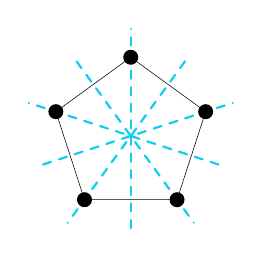
\begin{tikzpicture}
    \foreach \angle/\name in {-54/A,18/B,90/C,162/D,234/E} {
     \tkzDefPoint(\angle:1){\name}
    }
    \foreach \p/\q in {A/B,B/C,C/D,D/E,E/A} {
     \tkzDefMidPoint(\p,\q)
     \tkzGetPoint{S_\p\q}
    }
    \tkzDefPoint(0,0){O}
    \tkzDrawPolygon(A,B,C,D,E)
    \tkzDrawLine[thick,color=PolygonCyan,dashed](S_EA,C)
    \tkzDrawLine[thick,color=PolygonCyan,dashed](S_AB,D)
    \tkzDrawLine[thick,color=PolygonCyan,dashed](S_BC,E)
    \tkzDrawLine[thick,color=PolygonCyan,dashed](S_CD,A)
    \tkzDrawLine[thick,color=PolygonCyan,dashed](S_DE,B)
    \tkzDrawPoints(A,B,C,D,E)
   \end{tikzpicture}
  \end{subfigure}

  \caption*{Examples of regular polygon symmetries}
 \end{figure}
\end{frame}

\section{Cryptography on Regular Polygons}

\begin{frame}
 \frametitle{Chaining Symmetries}
 Given two symmetries, $s_1$ and $s_2$ of a regular polygon, one can apply them
 one after the other (`compose' them, like functions).\\
 \pause
 We'll denote this composition simply by $s_1s_2$.
\end{frame}

\begin{frame}
 \frametitle{Chaining Symmetries -- Example}
 \begin{figure}[H]
  \centering
  \begin{subfigure}[b]{\textwidth}
   \centering
   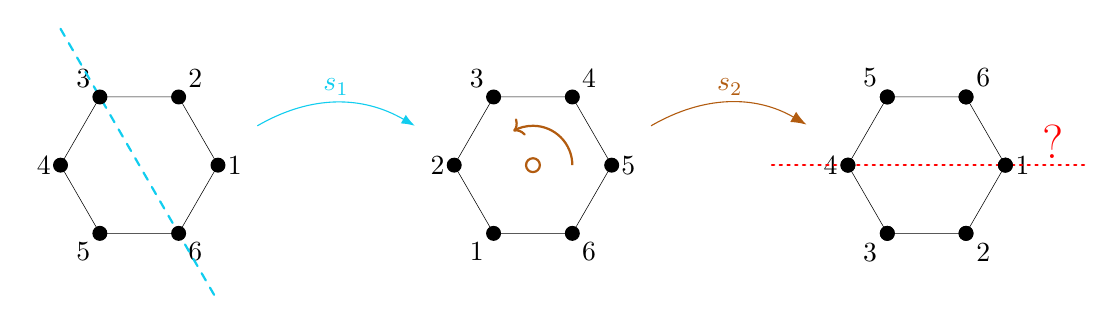
\begin{tikzpicture}
    \foreach \an/\name in {0/a,60/b,120/c,180/d,240/e,300/f} {
     \tkzDefPoint(\an:1){\name}
    }
    \tkzDrawPolygon(a,b,c,d,e,f)
    \tkzLabelPoint[right](a){$1$}
    \tkzLabelPoint[above right](b){$2$}
    \tkzLabelPoint[above left](c){$3$}
    \tkzLabelPoint[left](d){$4$}
    \tkzLabelPoint[below left](e){$5$}
    \tkzLabelPoint[below right](f){$6$}

    \tkzDrawLine[dashed,thick,PolygonCyan,add=.5 and .5](c,f)
    \tkzDrawPoints(a,b,c,d,e,f)

    \coordinate (h1) at ($(a) + (0.5,0.5)$);
    \coordinate (h2) at ($(h1) + (2,0)$);
    
    \pause
    \draw[PolygonCyan,-Latex,bend left=30] (h1) to
     node[midway,PolygonCyan,yshift=2mm] {$s_1$} (h2);

    \tkzDefPoint(6,0){a1}
    \tkzDefPointsBy[translation=from a to a1](b,c,d,e,f){b1,c1,d1,e1,f1}
    \tkzDrawPolygon(a1,b1,c1,d1,e1,f1)
    \tkzLabelPoint[right](a1){$5$}
    \tkzLabelPoint[above right](b1){$4$}
    \tkzLabelPoint[above left](c1){$3$}
    \tkzLabelPoint[left](d1){$2$}
    \tkzLabelPoint[below left](e1){$1$}
    \tkzLabelPoint[below right](f1){$6$}
    \tkzDrawPoints(a1,b1,c1,d1,e1,f1)

    \tkzDefPoint(5,0){o}
    \tkzDrawPoint[fill=none,PolygonOrange,thick](o)
    \tkzDrawArc[R,thick,PolygonOrange,->](o,0.5)(0,120)

    \coordinate (g1) at ($(a1) + (0.5,0.5)$);
    \coordinate (g2) at ($(g1) + (2,0)$);

    \pause
    \draw[PolygonOrange,-Latex,bend left=30] (g1) to
     node[midway,PolygonOrange,yshift=2mm] {$s_2$} (g2);

    \tkzDefPoint(11,0){a2}
    \tkzDefPointsBy[translation=from a1 to a2](b1,c1,d1,e1,f1){b2,c2,d2,e2,f2}
    \tkzDrawPolygon(a2,b2,c2,d2,e2,f2)
    \tkzLabelPoint[right](a2){$1$}
    \tkzLabelPoint[above right](b2){$6$}
    \tkzLabelPoint[above left](c2){$5$}
    \tkzLabelPoint[left](d2){$4$}
    \tkzLabelPoint[below left](e2){$3$}
    \tkzLabelPoint[below right](f2){$2$}
    \tkzDrawPoints(a2,b2,c2,d2,e2,f2)

    \pause
    \tkzDrawLine[thick,dotted,add=.5 and .5,Red](a2,d2)
    \tkzLabelLine[pos=-0.3,Red,yshift=3mm](a2,d2){\LARGE $?$}
    \tkzDrawPoints(a2,b2,c2,d2,e2,f2)
   \end{tikzpicture}
  \end{subfigure}
  \caption*{Example of a chain of symmetries.}
 \end{figure}
\end{frame}

\begin{frame}
 \frametitle{Chaining Symmetries -- How Many Do We Need?}
 Discounting point symmetry, an $n$-gon has \alert{$2n$} symmetries.\\
 \pause
 Two symmetries can `combine' to create a different symmetry.\\
 \pause
 \textbf{Natural question:} How many (and which) symmetries of a regular polygon
  do I need to get all the others?\\
  \pause
  For example,
  \begin{itemize}[label=\textbullet,topsep=0pt]
   \item if $s_1$ is any reflectional symmetry and $s_2$ is a rotation by $60^{
    \circ }$ counter-clockwise, then $s_2^3s_1$ ($s_2^3$ means $s_2s_2s_2$)
    reflects a hexagon through a line perpendicular to the line of $s_1$.
   \pause
   \item if $s_1$ is a rotation by $120^{ \circ }$ clockwise and $s_2$ is a
    reflection through a vertical line passing through the top vertex, then
    $s_1s_2$ is a reflection through the line given by the rotation of the line
    of $s_2$ $60^{ \circ }$ clockwise.
  \end{itemize}
\end{frame}

\begin{frame}
 \frametitle{Chaining Symmetries -- How Many Do We Need?}
 Actually, for a general $n$-gon, we need only \alert{two}:
 \pause
 \begin{itemize}[label=\textbullet,topsep=0pt]
  \item rotation by $360^{ \circ } / n$ in any direction (we'll denote it $r$),
  \pause
  \item any reflection (we'll denote it $s$).
 \end{itemize}
\end{frame}

\begin{frame}
 \frametitle{Chaining Symmetries -- Triangle}
 Let $r$ be the rotation by $120^{ \circ }$ and $s$ any reflectional symmetry.\\
 \pause
 \begin{itemize}[label=\textbullet]
  \item The other two rotational symmetries are $r^2$ and $r^3$.
  \pause
  \item The other two reflectional symmetries are $rs$ and $r^2s$.
  \pause
  \item Therefore, all the symmetries of an equilateral triangle are
  \[
   \{r,r^2,r^3,s,rs,r^2s\}.
  \]
 \end{itemize}
\end{frame}

\begin{frame}
 \frametitle{Chaining Symmetries -- General Algorithm} In general, to create all
 symmetries, one needs a rotation by an angle $k \cdot 360^{ \circ }/n$ where
 $k$ \alert{doesn't share a prime factor} with $n$ (in other words, the fraction
 $\frac{k}{n}$ cannot be simplified) and any one reflectional symmetry. \\
 \pause
 \textbf{Why?}
 \begin{itemize}[label=\textbullet,topsep=0pt]
  \item<2-> If $k$ shares factors with $n$, then you can never get rotation by
   $360^{ \circ }/n$.
  \item<3-> Two symmetries cannot in general produce every rotation.
  \item<4-> Two rotations can never produce a symmetry.
 \end{itemize}
\end{frame}

\begin{frame}
 \frametitle{Chaining Symmetries -- General Algorithm}
 You're given a rotation $\clc{r}$ by $k \cdot 360^{ \circ }/n$ such that $k$
 doesn't share factors with $n$ and a reflectional symmetry $\clo{s}$.\\
 \pause
 \vspace{1em}
 \begin{block}{If you need to calculate a \textbf{rotation}, then}
  \begin{enumerate}[topsep=0pt]
   \item<2-> First measure the angle \textbf{counter-clockwise}.
   \item<3-> Find $a$ such that $\clc{r}^{a}$ is the rotation by $360^{ \circ }/n$.
   \item<4-> Then, find $b$ such that $(\clc{r}^{a})^{b} = \clc{r}^{ab}$ is your
    desired rotation.
  \end{enumerate}
 \end{block}
\end{frame}

\begin{frame}
 \frametitle{Chaining Symmetries -- General Algorithm}
 You're given a rotation $\clc{r}$ by $k \cdot 360^{ \circ }/n$ such that $k$
 doesn't share factors with $n$ and a line symmetry $\clo{s}$.\\
 \vspace{1em}
 \pause
 \begin{block}{If you need to calculate a \textbf{reflection}, then}
  \begin{enumerate}[topsep=0pt]
   \item Find $a$ such that $\clc{r}^{a}$ is the rotation by $360^{ \circ }/n$.
   \pause
   \item Determine the angle \textbf{in any direction} between the lines of your
    given reflection $\clo{s}$ and the reflection you want.
   \pause
   \item Find $b$ such that $\clc{r}^{ab}$ is a rotation \textbf{in the
    opposite direction} by \alert{twice} the angle from the previous step.
   \pause
   \item $\clc{r}^{ab}\clo{s}$ is your desired reflection.
  \end{enumerate}
 \end{block}
 \pause
 \textbf{\clo{Voluntary HW: }}\emph{Why} does this algorithm work?
\end{frame}

\begin{frame}
 \frametitle{Chaining Symmetries -- Algorithm Example}
 We're given two symmetries of the square:
 \vspace*{-1em}
 \begin{figure}[H]
  \centering
  \begin{subfigure}[b]{.4\textwidth}
   \centering
   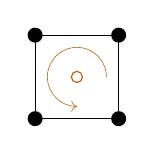
\begin{tikzpicture}[scale=0.75]
    \foreach \an/\name in {-45/a,45/b,135/c,-135/d} {
     \tkzDefPoint(\an:1){\name}
    }
    \tkzDrawPolygon(a,b,c,d)
    \tkzDrawPoints(a,b,c,d)
 
    \tkzDefPoint(0,0){o}
    \tkzDrawPoint[PolygonOrange,fill=none,size=4](o)
    \tkzDrawArc[R,PolygonOrange,->](o,0.5)(0,270)
   \end{tikzpicture}
   \vspace*{-6pt}
   \caption*{rotation \clo{r} by $270^{ \circ }$}
  \end{subfigure}
  \begin{subfigure}[b]{.4\textwidth}
   \centering
   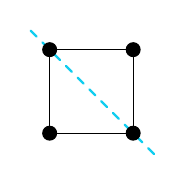
\begin{tikzpicture}[scale=0.75]
    \foreach \an/\name in {-45/a,45/b,135/c,-135/d} {
     \tkzDefPoint(\an:1){\name}
    }
    \tkzDrawPolygon(a,b,c,d)

    \tkzDrawLine[PolygonCyan,dashed,thick,add=.25 and .25](a,c)
    \tkzDrawPoints(a,b,c,d)
   \end{tikzpicture}
   \vspace*{-6pt}
   \caption*{reflection \clc{s} over the \clc{first diagonal}}
  \end{subfigure}
 \end{figure}
 \vspace*{-2em}
 and want to produce
 \begin{figure}[H]
  \centering
  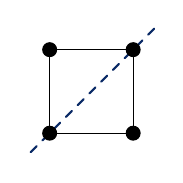
\begin{tikzpicture}[scale=0.75]
   \foreach \an/\name in {-45/a,45/b,135/c,-135/d} {
    \tkzDefPoint(\an:1){\name}
   }
   \tkzDrawPolygon(a,b,c,d)
 
   \tkzDrawLine[PolygonBlue,dashed,thick,add=.25 and .25](b,d)
   \tkzDrawPoints(a,b,c,d)
  \end{tikzpicture}
  \vspace*{-6pt}
  \caption*{reflection over the \clb{second diagonal}}
 \end{figure}
\end{frame}

\begin{frame}
 \frametitle{Chaining Symmetries -- Algorithm Example}
 We're given two symmetries of the square: rotation $\clo{r}$ by $270^{ \circ }$
 counter-clockwise and reflection $\clc{s}$ over the first diagonal.\\
 How to produce \clb{reflection over the other diagonal?}\\
 \pause
 \vspace{1em}
 \begin{block}{We use the algorithm.}
  \begin{enumerate}
   \item Repeating $\clo{r}$ three times gives the rotation by $90^{ \circ }$
    counter-clockwise, that is, $a = 3$.
   \pause
   \item The angle between the two diagonals is $90^{ \circ }$ in any direction.
   \pause
   \item Repeating the rotation from step 1 two times (that is, $b = 2$) and
    then using $\clc{s}$ gives the desired symmetry -- in this case it's
    $(\clo{r}^3)^2 \clc{s} = \clo{r}^{6} \clc{s}$. Of course, $\clo{r}^{4}$ is
    rotation by $360^{ \circ }$ which does nothing, so the final symmetry is
    $\clo{r}^2 \clc{s}$.
  \end{enumerate}
 \end{block}
\end{frame}

\subsection{Encoding Messages Using Symmetries}
\begin{frame}
 \subsectionpage
\end{frame}

\begin{frame}
 \frametitle{Encoding Messages -- General Idea}
 \begin{itemize}[label=\textbullet]
  \item Send a message as a sequence of strings which \alert{can be decoded on
   the other side}.
  \pause
  \item The decoding should require a `key' which is \alert{statistically
   impossible to determine quickly}.
  \pause
  \item The encoding and decoding must be done procedurally -- requires a system
   with concrete rules and a \alert{limited} (but huge) \alert{number of
   combinations}.
 \end{itemize}
\end{frame}

\begin{frame}
 \frametitle{Encoding Messages -- Regular Polygons}
 How can one use regular polygons to encode messages?\\
 \pause
 Quite easily, assign symbols to vertices and choose one \alert{main} vertex.\\
 \pause
 The symbol in the \alert{main} vertex is what is sent during each tick (time
 interval during which symbols are sent).\\
 \pause
 Rotations and reflections `move symbols between vertices'.\\
 \pause
 This means that after applying a rotation or reflection, a (in most cases)
 different symbol will appear in the main vertex.
\end{frame}

\begin{frame}
 \frametitle{Encoding Messages -- Morse Code}
 The Morse Code has two symbols: $-$ and $ \cdot $.\\
 \pause
 We also need to be able to determine spaces between words -- we can assign one
 vertex a `blank', meaning space.\\
 \pause
 This means that to send messages written Morse Code using regular polygons, we
 need three vertices -- a triangle.
\end{frame}

\begin{frame}
 \frametitle{Encoding Messages -- Morse Code}
 Let the top vertex be main and let's choose a rotation $r = \circlearrowleft
 120^{ \circ }$ and a reflection $s$ depicted below.\\
 \pause
 We should also assign Morse Code symbols to two of the vertices. We can do so
 randomly.
 \pause
 \begin{center}
  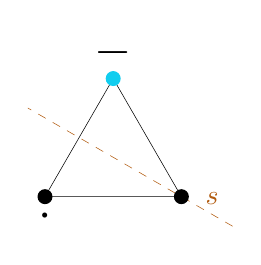
\begin{tikzpicture}
   \tkzDefPoint(-30:1){a}
   \tkzDefPoint(90:1){b}
   \tkzDefPoint(210:1){c}

   \tkzDrawPolygon(a,b,c)

   \tkzLabelPoint[above](b){\LARGE $-$}
   \tkzLabelPoint[below](c){\LARGE $ \cdot $}
   \tkzDefMidPoint(b,c) \tkzGetPoint{sbc}
   \tkzDrawLine[PolygonOrange,dashed,add=.5 and .5](a,sbc)
   \tkzLabelLine[pos=-0.3,above,PolygonOrange](a,sbc){$s$}

   \tkzDrawPoints(a,c)
   \tkzDrawPoint[PolygonCyan](b)
  \end{tikzpicture}
 \end{center}
 \pause
 The \clc{top vertex} is the main one, which means that the symbol above it will
 get sent.
\end{frame}

\begin{frame}
 \frametitle{Encoding Messages -- Morse Code}
 The important property of symmetries is that two different sequences can give
 the same symmetry.
 \pause
 Meaning, we can encode one message \alert{MANY} different ways.\\
 \pause
 For example, we can send the letter P ($ \cdot - - \, \cdot $) like this:
 \begin{center}
  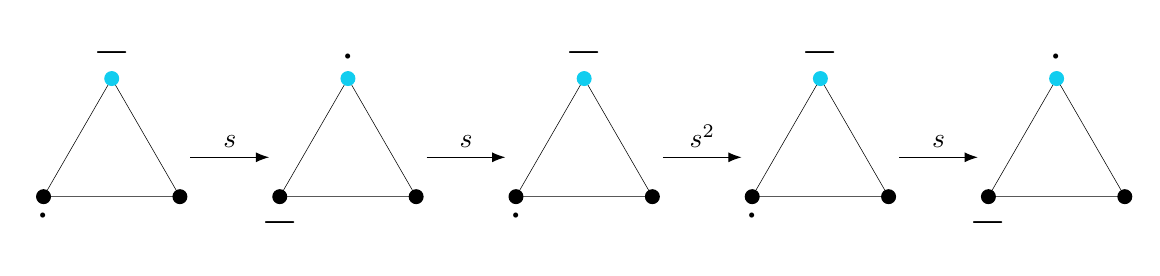
\begin{tikzpicture}
   \tkzDefPoint(0,0){t1}
   \tkzDefPoint(-30:1){a1}
   \tkzDefPoint(90:1){b1}
   \tkzDefPoint(210:1){c1}

   \tkzDrawPolygon(a1,b1,c1)
   \tkzLabelPoint[above](b1){\LARGE $-$}
   \tkzLabelPoint[below](c1){\LARGE $ \cdot $}

   \tkzDrawPoints(a1,c1)
   \tkzDrawPoint[PolygonCyan](b1)

   \tkzDefPoint(3,0){t2}
   \tkzDefPointsBy[translation= from t1 to t2](a1,b1,c1){a2,b2,c2}

   \tkzDrawPolygon(a2,b2,c2)
   \tkzLabelPoint[above](b2){\LARGE $ \cdot $}
   \tkzLabelPoint[below](c2){\LARGE $ - $}

   \tkzDrawPoints(a2,c2)
   \tkzDrawPoint[PolygonCyan](b2)

   \tkzDefPoint(6,0){t3}
   \tkzDefPointsBy[translation= from t2 to t3](a2,b2,c2){a3,b3,c3}

   \tkzDrawPolygon(a3,b3,c3)
   \tkzLabelPoint[above](b3){\LARGE $ - $}
   \tkzLabelPoint[below](c3){\LARGE $ \cdot $}

   \tkzDrawPoints(a3,c3)
   \tkzDrawPoint[PolygonCyan](b3)

   \tkzDefPoint(9,0){t4}
   \tkzDefPointsBy[translation= from t3 to t4](a3,b3,c3){a4,b4,c4}

   \tkzDrawPolygon(a4,b4,c4)
   \tkzLabelPoint[above](b4){\LARGE $ - $}
   \tkzLabelPoint[below](c4){\LARGE $ \cdot $}

   \tkzDrawPoints(a4,c4)
   \tkzDrawPoint[PolygonCyan](b4)

   \tkzDefPoint(12,0){t5}
   \tkzDefPointsBy[translation= from t3 to t4](a4,b4,c4){a5,b5,c5}

   \tkzDrawPolygon(a5,b5,c5)
   \tkzLabelPoint[above](b5){\LARGE $ \cdot $}
   \tkzLabelPoint[below](c5){\LARGE $ - $}

   \tkzDrawPoints(a5,c5)
   \tkzDrawPoint[PolygonCyan](b5)

   \draw[-Latex] ($(t1.center) + (1,0)$) to node[midway,yshift=2mm] {$s$}
    ($(t2.center) - (1,0)$);
   \draw[-Latex] ($(t2.center) + (1,0)$) to node[midway,yshift=2mm] {$s$}
    ($(t3.center) - (1,0)$);
   \draw[-Latex] ($(t3.center) + (1,0)$) to node[midway,yshift=2.7mm] {$s^2$}
    ($(t4.center) - (1,0)$);
   \draw[-Latex] ($(t4.center) + (1,0)$) to node[midway,yshift=2mm] {$s$}
    ($(t5.center) - (1,0)$);
  \end{tikzpicture}
 \end{center}
 \pause
 Or, as a sequence
 \[
  s,s,s^2,s.
 \]
\end{frame}

\begin{frame}
 \frametitle{Encoding Messages -- Morse Code}
 Notice that we didn't need the rotation $r$ at all in this example.\\
 \pause
 However, that doesn't mean we \alert{can't} use it.\\
 \pause
 Actually, it's often beneficial to encode messages using different combinations
 of symmetries for security.\\
 \pause
 The letter $ \cdot - - \, \cdot $ can also be sent for example like this
 \[
  r^2,sr,s r^2,rs r.
 \]
\end{frame}

\begin{frame}
 \frametitle{Encoding Messages -- Alphabet}
 The English alphabet has 26 letters, meaning we need a $27$-gon to represent
 all of them together with a blank.\\
\end{frame}

\begin{frame}
 \frametitle{Encoding Messages -- Alphabet}
 \vspace*{-1em}
 \begin{minipage}{.6\textwidth}
  \begin{center}
   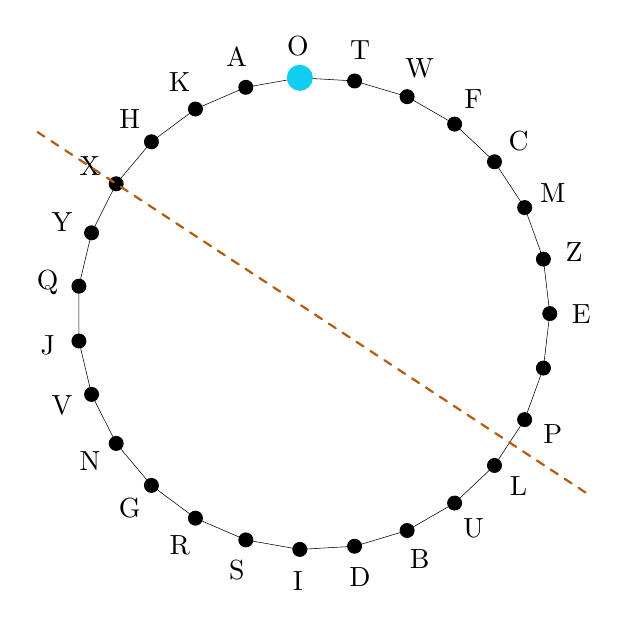
\begin{tikzpicture}
    \foreach \i in {0,1,...,26} {
     \tkzDefPoint({\i * 360 / 27}:3){p\i}
    }
    \tkzDrawPolygon(p0,p1,p2,p3,p4,p5,p6,p7,p8,p9,p10,p11,p12,p13,p14,p15,p16,p17,p18,p19,p20,p21,p22,p23,p24,p25,p26)
    \tkzDrawPoints(p0,p1,p2,p3,p4,p5,p6,p7,p8,p9,p10,p11,p12,p13,p14,p15,p16,p17,p18,p19,p20,p21,p22,p23,p24,p25,p26)
    \tkzDrawPoint[size=9,PolygonCyan](p7)

    \foreach \i/\letter in
    {0/E,1/Z,2/M,3/C,4/F,5/W,6/T,7/O,8/A,9/K,10/H,11/X,12/Y,13/Q,14/J,15/V,16/N,17/G,18/R,19/S,20/I,21/D,22/B,23/U,24/L,25/P} {
     \node at ({\i * 360 / 27}:3.4) {\letter};
    }
    \tkzDefMidPoint(p24,p25) \tkzGetPoint{slp}
   \tkzDrawLine[PolygonOrange,thick,dashed](p11,slp)
   \end{tikzpicture}
  \end{center}
 \end{minipage}
 \pause
 \begin{minipage}{.39\textwidth}
  Let's start with $r = \circlearrowleft \frac{2}{27} \cdot 360^{ \circ }$ and
  $\clo{s}$ as on the picture.\\
  \pause
  One way to encode the word POLYGONS would be
  \[
   s r^{5},r^{10}s r^{15},r^{5},s r,r^{7}s,r^{5}s r^{13},s r,r^3 s
  \]
  
 \end{minipage}
\end{frame}

\end{document}
